\documentclass[11pt]{article}
\title{Eigenmath Manual}
%\author{George Weigt}
\date{\today}
\usepackage{graphicx}
\usepackage{makeidx}
\makeindex

\begin{document}

\maketitle

\newpage


\newpage

%The symbol {\tt\char32} indicates a mandatory space.

\begin{center}
\begin{tabular}{clll}
{\it Math} & & {\it Eigenmath} & {\it Alternate form and/or comment} \\
\\
$-a$ & & {\tt -a} \\
\\
$a+b$ & & {\tt a+b} \\
\\
$a-b$ & & {\tt a-b} \\
\\
$ab$ & & {\tt a*b} & \verb$a b$ \hspace{10pt}
{\it with a space in between} \\
\\
$\displaystyle{a\over b}$ & & {\tt a/b} \\
\\
$\displaystyle{a\over bc}$ & & {\tt a/b/c} \\
\\
$a^2$ & & {\tt a{\char94}2} \\
\\
$\sqrt{a}$ & & {\tt a{\char94}(1/2)} & {\tt sqrt(a)} \\
\\
$\displaystyle{1\over\sqrt a}$ & & {\tt a{\char94}(-1/2)} & {\tt 1/sqrt(a)} \\
\\
$a(b+c)$ & & {\tt a*(b+c)} & \verb$a (b+c)$
\hspace{10pt} {\it with a space in between} \\
\\
$f(a)$ & & {\tt f(a)} \\
\\
$\displaystyle{\left(\matrix{a\cr b\cr c\cr}\right)}$ & & {\tt (a,b,c)} \\
\\
$\displaystyle{\left(\matrix{a&b\cr c&d\cr}\right)}$ & & {\tt ((a,b),(c,d))} \\
\\
$T^{12}$ & & {\tt T[1,2]} & {\it tensor component access} \\
\\
$2\,\rm km$ & & {\tt 2*"km"} & {\it units of measure should be quoted} \\
\end{tabular}
\end{center}


\newpage

\chapter{The Big Picture}
Let us begin by considering the following passage from Vladimir Nabokov's
autobiography {\it Speak, Memory.}

\medskip
\noindent
``A foolish tutor had explained logarithms to me much too early, and I had
read (in a British publication, the {\it Boy's Own Paper}, I believe)
about a certain Hindu calculator who in exactly two seconds could find the
seventeenth root of, say,
3529471145760275132301897342055866171392
(I am not sure I have got this right; anyway the root was 212).''

\medskip
\noindent
We can check Nabokov's arithmetic by typing the following into Eigenmath.

\medskip
\verb$212^17$

\medskip
\noindent
After pressing the return key we should get the following result.
$$3529471145760275132301897342055866171392$$
So Nabokov did get it right after all.
We can enter {\it float} or click on the float button to scale the number
down to size.

\medskip
\verb$float$

$$3.52947\times10^{39}$$



\noindent
There is a proposal to define Avogadro's constant as exactly $84446886^3$
atoms or molecules.\footnote{Fox, Ronald and Theodore Hill.
``An Exact Value for Avogadro's Number.''
{\it American Scientist} 95 (2007): 104--107.
The proposed number in the article is actually $84446888^3$.
In a subsequent addendum the authors reduced it to $84446886^3$ to be divisible
by 12. See {\tt www.physorg.com/news109595312.html}}
Of course, this number corresponds to a perfect cube of material with 84446886
atoms along each edge.
Let us check the difference between the proposed value and the measured value
of $(6.0221415\pm0.0000010)\times10^{23}$ atoms.

\medskip
\verb$A=84446886^3$

\verb$B=6.0221415*10^23$

\verb$A-B$

$$-5.17173\times10^{16}$$

\verb$0.0000010*10^23$

$$1\times10^{17}$$

\medskip
\noindent
We see that the proposed value is within the experimental error.
Just for the fun of it, let us factor the proposed value.

\medskip
\verb$factor(A)$

$$2^3\times3^3\times1667^3\times8443^3$$



\noindent
It is a generally accepted convention that $0^0=1$.
By drawing a graph of the function $f(x)=|x^x|$ we can see why this
convention makes sense.
Of course, we want to draw the absolute value, or magnitude of $x^x$ because
$x^x$ is mostly complex when $x<0$.

\medskip
\verb$f=abs(x^x)$

\verb$xrange=(-2,2)$

\verb$yrange=(-2,2)$

\verb$draw(f)$

\begin{center}
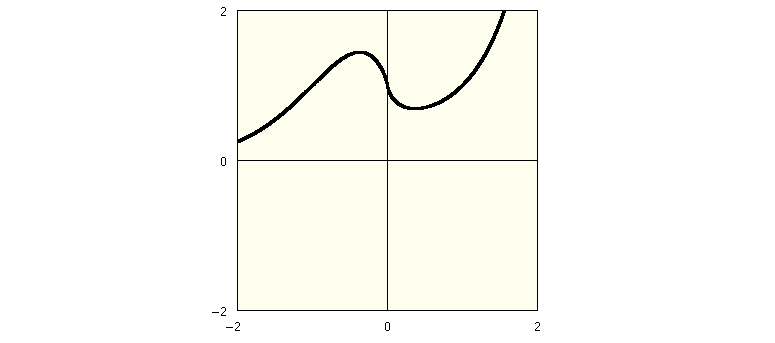
\includegraphics[scale=0.4]{zerozero.png}
\end{center}

\medskip
\noindent
We can see how $0^0=1$ results in a continuous line through $x=0$.

% What are the coordinates for the local minimum and maximum seen above?


\section*{Geometric series}

A geometric series converges according to the formula
$$\sum_{k=0}^\infty a^k={1\over1-a},\qquad|a|<1$$
If we use $a=-1/2$ and for practical purposes only count up to nine instead of infinity,
we should have
$$\sum_{k=0}^9\left(-{1\over2}\right)^k\approx{2\over3}$$
The above calculation can be done in one line of code using the $sum$ function.

\medskip
\verb$sum(k,0,9,(-0.5)^k)$
$$0.666016$$

\medskip
\noindent
The following example uses an intermediate variable.

\medskip
\verb$f=sum(k,0,9,a^k)$

\verb$f$
$$f=1+a+a^2+a^3+a^4+a^5+a^6+a^7+a^8+a^9$$

\verb$eval(f,a,-1/2)$
$$341\over512$$

\verb$float(last)$
$$0.666016$$

\medskip
\noindent
As seen on the first line, no result is printed when a symbol is defined.
When you do in fact want to see the value of a symbol,
just enter it as shown on the second line.

\medskip
\noindent
When a result is displayed, it is also stored in the symbol $last$.

\newpage

\noindent
The following example shows how to define a function.

\medskip
\verb$f(a)=sum(k,0,9,a^k)$

\verb$f$
$$f=\mathop{\rm sum}(k,0,9,a^k)$$

\verb$f(-1/2)$
$$341\over512$$

\verb$f(-0.5)$
$$0.666016$$

\medskip
\noindent
Eigenmath handles function definitions in a special way.
Unlike a normal symbol, a function definition is not evaluated immediately.
The following example demonstrates the difference.

\medskip
\verb$f=sum(k,0,9,a^k)$

\verb$f$
$$f=1+a+a^2+a^3+a^4+a^5+a^6+a^7+a^8+a^9$$

\verb$f(a)=sum(k,0,9,a^k)$

\verb$f$
$$f=\mathop{\rm sum}(k,0,9,a^k)$$

\medskip
\noindent
Why are they handled differently?
Well, suppose we want to define $f$ as a function of two variables,
$a$ and $n$, like this.

\medskip
\verb$f(a,n)=sum(k,0,n,a^k)$

\medskip
\noindent
In this case it is not possible to evaluate the sum right away.
The value of $n$ will not be known until $f$ is actually used somewhere.
Consequently, Eigenmath does not normally evaluate a function when it is defined.
Now, having said that, there are two work arounds that provide exceptions to the rule.
They are {\it eval} and {\it quote}.
 
\medskip
\verb$f=quote(sum(k,0,9,a^k))$

\verb$f$
$$f=\mathop{\rm sum}(k,0,9,a^k)$$

\verb$f(a)=eval(sum(k,0,9,a^k))$

\verb$f$
$$f=1+a+a^2+a^3+a^4+a^5+a^6+a^7+a^8+a^9$$



\subsection{Units of measure}
\index{units of measure}
Quoted strings can be used to express units of measurement in a calculation.
For example, the space shuttle accelerates from zero to
17{,}000 miles per hour in 8 minutes.
The average acceleration of the space shuttle is

\medskip
\verb$v=17000*"mile"/"hr"$

\verb$t=8*"min"/(60*"min"/"hr")$

\verb$v/t$
$$127500\,\hbox{mile}\over(\hbox{hr})^2$$



\section*{Draw}
$draw(f,x)$ draws a graph of the function $f$ of $x$.
The second argument can be omitted when the dependent variable
is literally $x$ or $t$.
The vectors $xrange$ and $yrange$ control the scale of the graph.

\medskip
\verb$draw(x^2)$

\medskip
\begin{center}
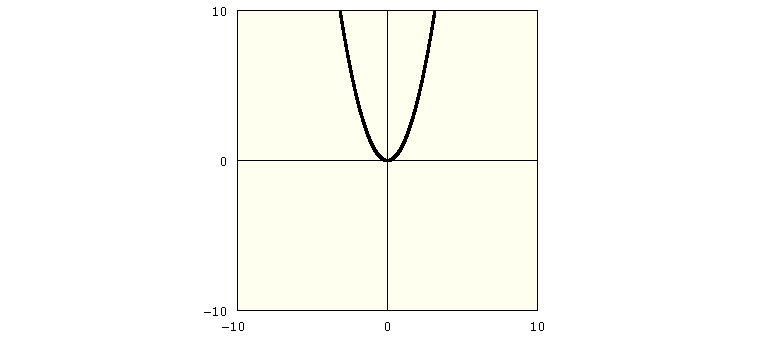
\includegraphics[scale=0.4]{parabola.png}
\end{center}

\verb$xrange=(-1,1)$

\verb$yrange=(0,2)$

\verb$draw(x^2)$

\medskip
\begin{center}
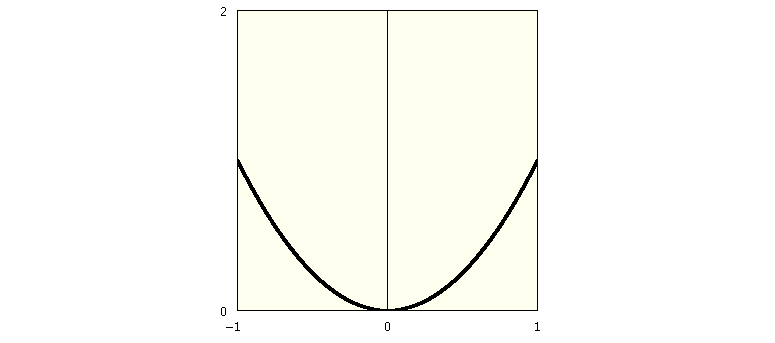
\includegraphics[scale=0.4]{parabola2.png}
\end{center}

\verb$clear$

\medskip
\noindent
The clear command (or a click of the Clear button)
resets $xrange$ and $yrange$.
This needs to be done so that the next graph
appears as shown.

\newpage

\noindent
Parametric drawing occurs when a function returns a vector.
The vector $trange$ controls the parameter range.
The default range is $(-\pi,\pi)$.

\medskip
\verb$f=(cos(t),sin(t))$

\verb$draw(5*f)$

\medskip
\begin{center}
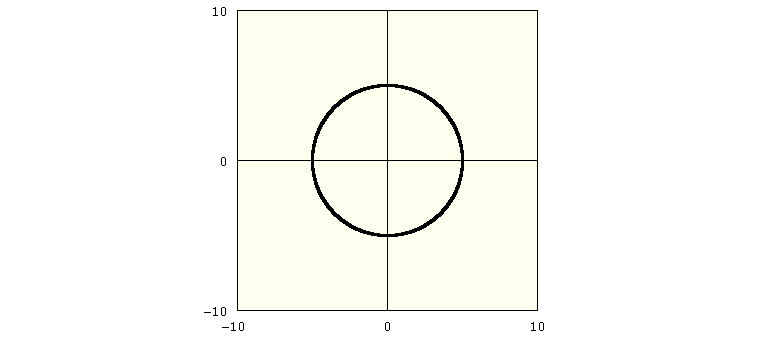
\includegraphics[scale=0.4]{circle.png}
\end{center}

\verb$trange=(0,pi/2)$

\verb$draw(5*f)$

\medskip
\begin{center}
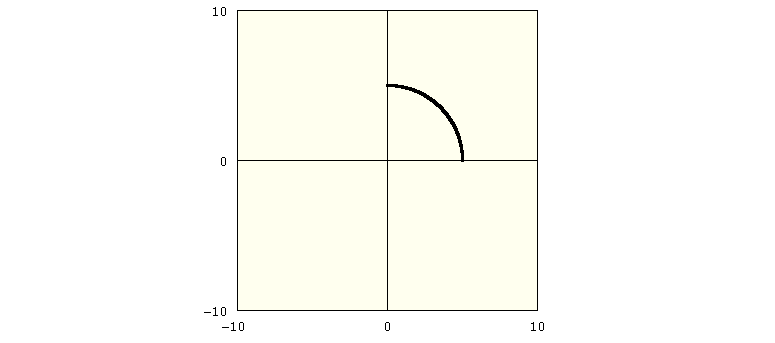
\includegraphics[scale=0.4]{circle2.png}
\end{center}

\newpage

\noindent
Here are a couple of interesting curves and the code for drawing them.
First is a lemniscate.

\medskip
\verb$clear$

\verb$X=cos(t)/(1+sin(t)^2)$

\verb$Y=sin(t)*cos(t)/(1+sin(t)^2)$

\verb$draw(5*(X,Y))$

\medskip
\begin{center}
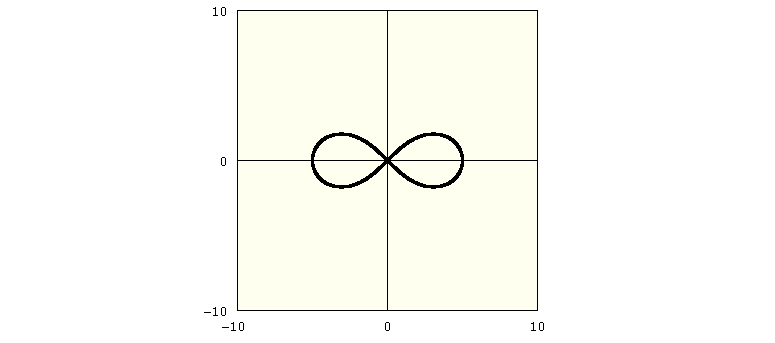
\includegraphics[scale=0.4]{lemniscate.png}
\end{center}

\medskip
\noindent
Next is a cardioid.

\medskip
\verb$r=(1+cos(t))/2$

\verb$u=(cos(t),sin(t))$

\verb$xrange=(-1,1)$

\verb$yrange=(-1,1)$

\verb$draw(r*u)$

\medskip
\begin{center}
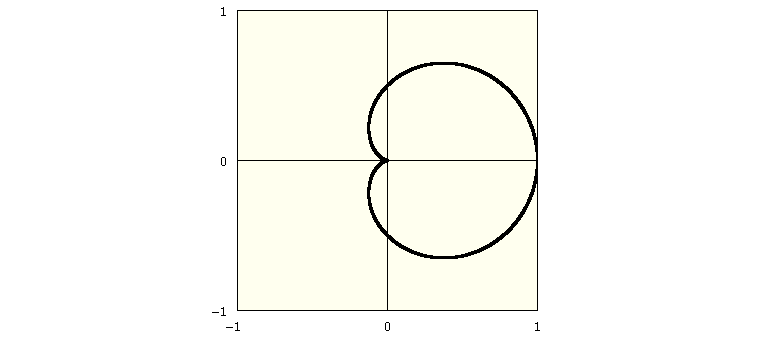
\includegraphics[scale=0.4]{cardioid.png}
\end{center}




\newpage

\index{scripting}

\noindent
Here is a simple example that draws the graph of $y=mx+b$.

\medskip
{\tt y=m*x+b}

{\tt m=1/2}

{\tt b=-3}

{\tt draw(y)}

\medskip
\noindent
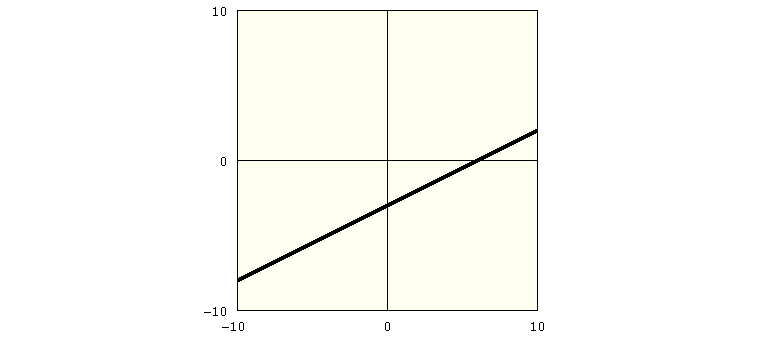
\includegraphics[scale=0.5]{1.png}

\newpage

\noindent
Now suppose that we want to draw the graph
with a different $m$.
We could type in everything all over again, but it would be easier
in the long run to write a script.
Then we can go back and quickly change $m$ and $b$ as many times as we want.

\medskip
\noindent
To prepare a script, click on the Edit Script button.
Then enter the script commands, one per line.

\medskip
{\tt y=m*x+b}

{\tt m=1/2}

{\tt b=-3}

{\tt draw(y)}

\medskip
\noindent
Next, click on the Run Script button to see the graph.

\medskip
\noindent
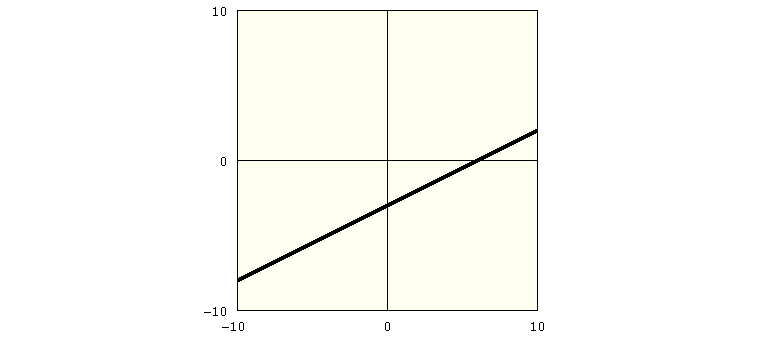
\includegraphics[scale=0.5]{1.png}

\medskip
\noindent
Eigenmath runs a script by stepping through it line by line.
Each line is evaluated just like a regular command.
This continues until the end of the script is reached.
After the script runs, you can click Edit Script and go back and change something.

\medskip
\noindent
By the way, Eigenmath automatically does a clear before
running a script.

\newpage

\noindent
Sometimes it is desirable to have a script print a few comments when it runs.
This can be accomplished by placing the desired text in quotes
on a single line.
For example, the script

\medskip
\verb$"Here is the value of pi."$

\verb$float(pi)$

\medskip
\noindent
displays the following when run.

\medskip
\verb$Here is the value of pi.$

$$3.14159$$



\section{Complex numbers}
When Eigenmath starts up, it defines the symbol $i$ as $i=\sqrt{-1}$.
Other than that, there is nothing special about $i$.
It is just a regular symbol that can be redefined and used for some other purpose if need be.

\medskip
\noindent
Complex quantities can be entered in rectangular or polar form.

\medskip
\verb$a+i*b$
$$a+ib$$

\verb$exp(i*pi/3)$
$$\exp({1\over3}i\pi)$$

\medskip
\noindent
Converting to rectangular or polar coordinates simplifies mixed forms.

\medskip
\verb$A=1+i$

\verb$B=sqrt(2)*exp(i*pi/4)$

\verb$A-B$
$$1+i-2^{1/2}\exp({1\over4}i\pi)$$

\verb$rect$
$$0$$

\medskip
\noindent
Rectangular complex quantities, when raised to a power, are multiplied out.

\medskip
\verb$(a+i*b)^2$
$$a^2-b^2+2iab$$

\medskip
\noindent
When $a$ and $b$ are numerical and the power is negative, the evaluation is done as follows.
$$(a+ib)^{-n}=\left[{a-ib\over(a+ib)(a-ib)}\right]^n=\left[{a-ib\over a^2+b^2}\right]^n$$
Of course, this causes $i$ to be removed from the denominator.
%For $n=1$ we have
%$${1\over a+ib}={a-ib\over a^2+b^2}$$
Here are a few examples.

\medskip
\verb$1/(2-i)$
$${2\over5}+{1\over5}i$$

\verb$(-1+3i)/(2-i)$
$$-1+i$$

\newpage

\noindent
The absolute value of a complex number returns its magnitude.

\medskip
\verb$abs(3+4*i)$
$$5$$

\medskip
\noindent
In light of this, the following result might be unexpected.

\medskip
\verb$abs(a+b*i)$
$$\mathop{\rm abs}(a+ib)$$

\medskip
\noindent
The result is not $\sqrt{a^2+b^2}$ because that would assume that
$a$ and $b$ are real.
For example, suppose that $a=0$ and $b=i$.
Then
$$|a+ib|=|-1|=1$$
and
$$\sqrt{a^2+b^2}=\sqrt{-1}=i$$
Hence
$$|a+ib|\ne\sqrt{a^2+b^2}\quad\hbox{for some $a,b\in\cal C$}$$

\medskip
\noindent
The {\it mag} function is an alternative.
It treats symbols like $a$ and $b$ as real.

\medskip
\verb$mag(a+b*i)$

$$(a^2+b^2)^{1/2}$$




\section{Linear algebra}
\index{linear algebra}
$dot$ is used to multiply vectors and matrices.
The following example shows how to use $dot$ and $inv$ to solve for
$\bf X$ in $\bf AX=B$.

\medskip
{\tt A=((3.8,7.2),(1.3,-0.9))}

{\tt B=(16.5,-22.1)}

{\tt X=dot(inv(A),B)}

{\tt X}

$$\left(\matrix{-11.2887\cr8.24961}\right)$$

\medskip
\noindent
One might wonder why the $dot$ function is necessary.
Why not simply use $X=inv(A)*B$ like scalar multiplication?
The reason is that the software normally reorders factors internally to optimize processing.
For example, $inv(A)*B$ in symbolic form is changed to $B*inv(A)$ internally.
Since the dot product is not commutative, this reordering would give the wrong result.
Using a function to do the multiply avoids the problem because
function arguments are not reordered.

\medskip
\noindent
It should be noted that $dot$ can have more than two arguments.
For example, $dot(A,B,C)$ can be used for the dot product of three tensors.

\bigskip
\noindent
The following example demonstrates the relation
${\bf A}^{-1}=\mathop{\rm adj}{\bf A}/\mathop{\rm det}{\bf A}$.

\medskip
\verb$A=((a,b),(c,d))$

\medskip
\verb$inv(A)$
$$\left(\matrix{
\displaystyle{d\over ad-bc} & \displaystyle{-{b\over ad-bc}}\cr
\cr
\displaystyle{-{c\over ad-bc}} & \displaystyle{a\over ad-bc}\cr
}\right)$$

\medskip
\verb$adj(A)$
$$\left(\matrix{
d & -b\cr
-c & a\cr
}\right)$$

\medskip
\verb$det(A)$
$$ad-bc$$

\medskip
\verb$inv(A)-adj(A)/det(A)$
$$\left(\matrix{
0 & 0\cr
0 & 0\cr
}\right)$$

\medskip
\noindent
Sometimes a calculation will be simpler if it can be reorganized to use $adj$ instead of $inv$.
The main idea is to try to prevent the determinant from appearing as a divisor.
For example, suppose for matrices $\bf A$ and $\bf B$ you want to check that
$${\bf A}-{\bf B}^{-1}=0$$
Depending on the complexity of $\mathop{\rm det}\bf B$, the software
may not be able to find a simplification that yields zero.
Should that occur, the following alternative can be tried.
$$(\mathop{\rm det}{\bf B})\cdot{\bf A}-\mathop{\rm adj}{\bf B}=0$$

\bigskip
\noindent
The adjunct of a matrix is related to the cofactors as follows.

\medskip
\verb$A=((a,b),(c,d))$

\verb$C=((0,0),(0,0))$

\verb$C[1,1]=cofactor(A,1,1)$

\verb$C[1,2]=cofactor(A,1,2)$

\verb$C[2,1]=cofactor(A,2,1)$

\verb$C[2,2]=cofactor(A,2,2)$

\verb$C$

$$C=\left(\matrix{d&-c\cr -b&a}\right)$$

\verb$adj(A)-transpose(C)$

$$\left(\matrix{0&0\cr0&0\cr}\right)$$





\section*{Calculus}
\index{derivative}
$d(f,x)$ returns the derivative of $f$ with respect to $x$.
The $x$ can be omitted for expressions in $x$.

\medskip
\verb$d(x^2)$
$$2x$$

\bigskip
\noindent
The following table summarizes the various ways to obtain multiderivatives.

\begin{center}
\begin{tabular}{cllllll}
%& & & & {\it alternate form} \\
%\\
$\displaystyle{\partial^2f\over\partial x^2}$ & & \verb$d(f,x,x)$ & & \verb$d(f,x,2)$ \\
\\
$\displaystyle{\partial^2f\over\partial x\,\partial y}$ & & \verb$d(f,x,y)$ \\
\\
$\displaystyle{\partial^{m+n+\cdot\cdot\cdot} f\over\partial x^m\,\partial y^n\cdots}$ & &
\verb$d(f,x,...,y,...)$ & & \verb$d(f,x,m,y,n,...)$ \\
\end{tabular}
\end{center}

%\medskip
%\verb$r=sqrt(x^2+y^2)$

%\verb$d(r,x,y)$
%$${-{xy\over(x^2+y^2)^{3/2}}}$$

\index{gradient}

\noindent
The gradient of $f$ is obtained by using a vector for $x$ in $d(f,x)$.

\medskip
\verb$r=sqrt(x^2+y^2)$

\verb$d(r,(x,y))$
$$\left(\matrix{
\displaystyle{{x\over(x^2+y^2)^{1/2}}}\cr
\cr
\displaystyle{{y\over(x^2+y^2)^{1/2}}}\cr
}\right)$$

\medskip
\noindent
The $f$ in $d(f,x)$ can be a tensor function.
Gradient raises the rank by one.

\medskip
\verb$F=(x+2y,3x+4y)$

\verb$X=(x,y)$

\verb$d(F,X)$
$$\left(\matrix{1&2\cr3&4}\right)$$

\newpage

\noindent
The function $f$ in $d(f)$ does not have to be defined.
It can be a template function with just a name and an argument list.
Eigenmath checks the argument list to figure out what to do.
For example, $d(f(x),x)$ evaluates to itself because $f$ depends on $x$.
However, $d(f(x),y)$ evaluates to zero because $f$ does not depend on $y$.

\medskip
\verb$d(f(x),x)$
$$\partial(f(x),x)$$

\verb$d(f(x),y)$
$$0$$

\verb$d(f(x,y),y)$
$$\partial(f(x,y),y)$$

\verb$d(f(),t)$
$$\partial(f(),t)$$

\medskip
\noindent
As the final example shows, an empty argument list causes
$d(f)$ to always evaluate to itself, regardless
of the second argument.

\medskip
\noindent
Template functions are useful for experimenting with differential forms.
For example, let us check the identity
$$\mathop{\rm div}(\mathop{\rm curl}{\bf F})=0$$
for an arbitrary vector function $\bf F$.

\medskip
\verb$F=(F1(x,y,z),F2(x,y,z),F3(x,y,z))$

\verb$curl(U)=(d(U[3],y)-d(U[2],z),d(U[1],z)-d(U[3],x),d(U[2],x)-d(U[1],y))$

\verb$div(U)=d(U[1],x)+d(U[2],y)+d(U[3],z)$

\verb$div(curl(F))$
$$0$$

\newpage

\index{integral}
$integral(f,x)$ returns the integral of $f$ with respect to $x$.
The $x$ can be omitted for expressions in $x$.
A multi-integral can be obtained by extending the argument list.

\medskip
\verb$integral(x^2)$
$${1\over3}x^3$$

\verb$integral(x*y,x,y)$
$${1\over4}x^2y^2$$

\medskip
\noindent
$defint(f,x,a,b,\ldots)$
computes the definite integral of $f$ with respect to $x$ evaluated from $a$ to $b$.
The argument list can be extended for multiple integrals.

\medskip
\noindent
The following example computes the integral of $f=x^2$
over the domain of a semicircle.
For each $x$ along the abscissa, $y$ ranges from 0 to $\sqrt{1-x^2}$.

\medskip
\verb$defint(x^2,y,0,sqrt(1-x^2),x,-1,1)$

$${1\over8}\pi$$

\medskip
\noindent
As an alternative, the $eval$ function can be used to compute a definite integral step by step.

\medskip
\verb$I=integral(x^2,y)$

\verb$I=eval(I,y,sqrt(1-x^2))-eval(I,y,0)$

\verb$I=integral(I,x)$

\verb$eval(I,x,1)-eval(I,x,-1)$
$${1\over8}\pi$$



\newpage

\noindent
Here is a useful trick.
Difficult integrals involving sine and cosine
can often be solved by using exponentials.
Trigonometric simplifications involving powers
and multiple angles turn into simple algebra in the
exponential domain.
For example, the definite integral
$$\int_0^{2\pi}\left(\sin^4t-2\cos^3(t/2)\sin t\right)dt$$
can be solved as follows.

\medskip
\verb$f=sin(t)^4-2*cos(t/2)^3*sin(t)$

\verb$f=circexp(f)$

\verb$defint(f,t,0,2*pi)$

$$-{16\over5}+{3\over4}\pi$$

\medskip
\noindent
Here is a check.

\medskip
\verb$g=integral(f,t)$

\verb$f-d(g,t)$

$$0$$



\begin{center}
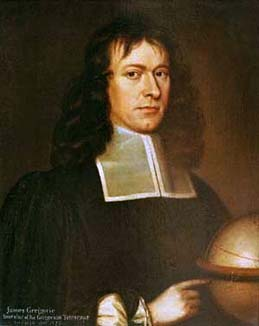
\includegraphics[]{JamesGregory.jpeg}
\end{center}

\bigskip

\noindent
James Gregory, a contemporary of Newton, was the first to publish the fundamental theorem of calculus.
$$\int_a^b f'(x)\,dx=f(b)-f(a)$$
Of course, the theorem is a formal expression of the inverse relation between integrals and derivatives.
On the next page is a simple example.

\newpage

\verb$f=x^2/2$

\verb$xrange=(-1,1)$

\verb$yrange=xrange$

\verb$draw(d(f))$

\noindent
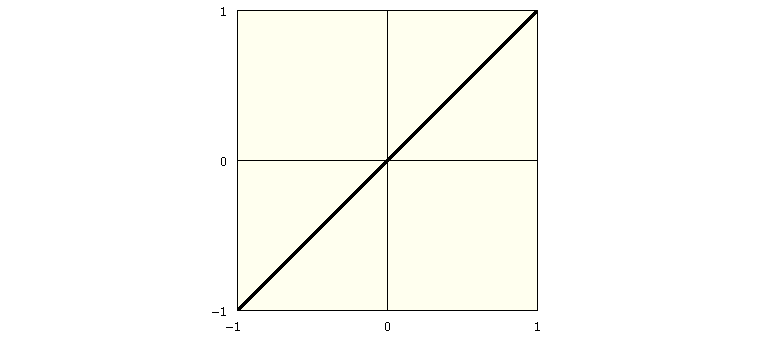
\includegraphics[scale=0.5]{funda1.png}

\verb$draw(integral(d(f)))$

\medskip
\noindent
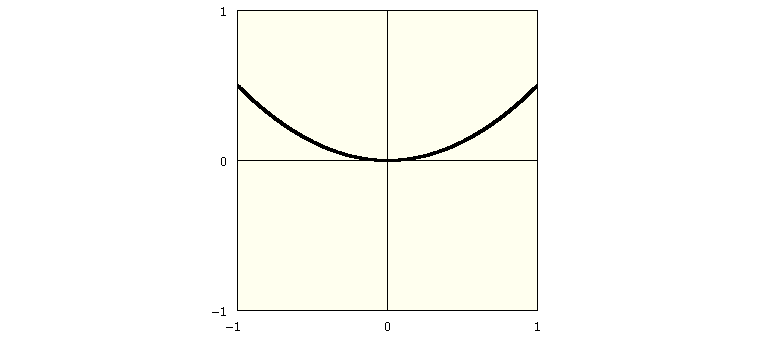
\includegraphics[scale=0.5]{funda2.png}

\medskip
\noindent
The first graph shows that the area under the curve $f'(x)$ is zero.
The second graph shows that $f(1)-f(-1)=0$.
Hence for $f(x)={1\over2}x^2$ we have
$$\int_{-1}^1f'(x)\,dx=f(1)-f(-1)=0$$




\subsection{Arc length}

Let $g(t)$ be a function that draws a curve.
The arc length from $g(a)$ to $g(b)$ is given by
$$\int_a^b|g'(t)|\,dt$$
where $|g'(t)|$ is the length of the tangent vector at $g(t)$.
The integral sums over all of the tangent lengths to arrive at the total length
from $a$ to $b$.
For example, let us measure the length of

\medskip
\verb$xrange=(0,1)$

\verb$yrange=(0,1)$

\verb$draw(x^2)$

\begin{center}
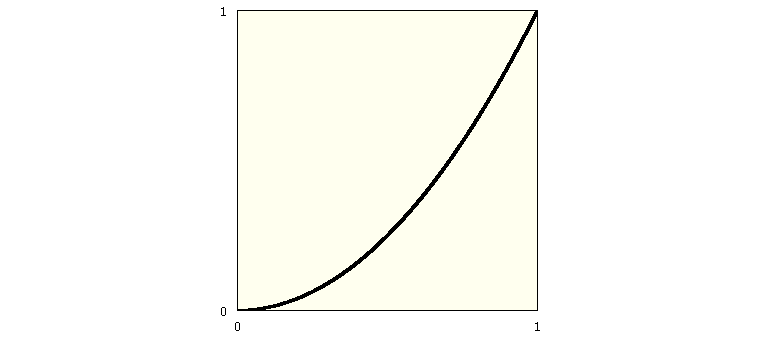
\includegraphics[scale=0.4]{arc.png}
\end{center}

\medskip
\noindent
A suitable $g(t)$ for the arc is
$$g(t)=(t,t^2),\quad0\le t\le1$$
The Eigenmath solution is

\medskip
\verb$g=(t,t^2)$

\verb$defint(abs(d(g,t)),t,0,1)$

$$\hbox{$1\over4$}\log(2+5^{1/2})+\hbox{$1\over2$}5^{1/2}$$

\verb$float$

$$1.47894$$

\medskip
\noindent
As we would expect, the result is greater than $\sqrt2$, the length of the
diagonal.

\medskip
\noindent
The result seems rather complicated given that we
started with a simple parabola.
Let us inspect $|g'(t)|$ to see why.

\medskip
\verb$g$

$$g=\left(\matrix{t\cr t^2}\right)$$

\medskip
\verb$d(g,t)$

$$\left(\matrix{1\cr2t}\right)$$

\medskip
\verb$abs(d(g,t))$

$$(4t^2+1)^{1/2}$$

\medskip
\noindent
The following script does a discrete computation of the arc length by dividing
the curve into 100 pieces.

\medskip
\verb$g(t)=(t,t^2)$

\verb$h(t)=abs(g(t)-g(t-0.01))$

\verb$L=0$

\verb$for(k,1,100,L=L+h(k/100.0))$

\verb$L$

$$L=1.47894$$

\newpage

\subsection{Line integrals}

There are two different kinds of line integrals,
one for scalar fields and one
for vector fields.
The following table shows how both are based on the calculation of
arc length.

\bigskip

\begin{center}
\begin{tabular}{|lll|}
\hline
 & & \\
& Abstract form
& Computable form
\\
 & & \\
Arc length
& $\displaystyle{\int_C ds}$
& $\displaystyle{\int_a^b |g'(t)|\,dt}$
\\
 & & \\
Line integral, scalar field
& $\displaystyle{\int_C f\,ds}$
& $\displaystyle{\int_a^b f(g(t))\,|g'(t)|\,dt}$
\\
 & & \\
Line integral, vector field
& $\displaystyle{\int_C(F\cdot u)\,ds}$
& $\displaystyle{\int_a^b F(g(t))\cdot g'(t)\,dt}$
\\
 & & \\
\hline
\end{tabular}
\end{center}

\bigskip
\noindent
For the vector field form, the symbol $u$ is the unit tangent vector
$$u={g'(t)\over|g'(t)|}$$
The length of the tangent vector cancels with $ds$
as follows.
$$\int_C(F\cdot u)\,ds
=\int_a^b\bigg(F(g(t))\cdot{g'(t)\over|g'(t)|}\bigg)\,\bigg(|g'(t)|\,dt\bigg)
=\int_a^b F(g(t))\cdot g'(t)\,dt
$$

\newpage

\noindent
Evaluate
$$\int_Cx\,ds\quad\hbox{and}\quad\int_Cx\,dx$$
where $C$ is a straight line from $(0,0)$ to $(1,1)$.

\medskip
\noindent
What a difference the measure makes.
The first integral is over a scalar field and the second is over a vector field.
This can be understood when we recall that
$$ds=|g'(t)|\,dt
%\quad\hbox{and}\quad
%\int_Cx\,dx=\int_Cx\,dx+0\,dy
$$
Hence for $\int_Cx\,ds$ we have

\medskip
\verb$x=t$

\verb$y=t$

\verb$g=(x,y)$

\verb$defint(x*abs(d(g,t)),t,0,1)$

$$1\over2^{1/2}$$

\medskip
\noindent
For $\int_Cx\,dx$ we have

\medskip
\verb$x=t$

\verb$y=t$

\verb$g=(x,y)$

\verb$F=(x,0)$

\verb$defint(dot(F,d(g,t)),t,0,1)$

$$1\over2$$

\newpage

\noindent
The following line integral problems are from
{\it Advanced Calculus, Fifth Edition} by Wilfred Kaplan.

\medskip
\noindent
Evaluate $\int y^2\,dx$ along the straight
line from $(0,0)$ to $(2,2)$.

\medskip
\verb$x=2t$

\verb$y=2t$

\verb$defint(y^2*d(x,t),t,0,1)$

$$8\over3$$

\medskip
\noindent
Evaluate $\int y\,dx$ along the straight line from
$(2,1)$ to $(1,2)$.

\medskip
\verb$x=2-t$

\verb$y=t+1$

\verb$defint(y*d(x),t,0,1)$

$$-{3\over2}$$

\medskip
\noindent
Evaluate $\int x\,dy$ along the straight line from
$(1,1)$ to $(2,1)$.

\medskip
\verb$x=t+1$

\verb$y=1$

\verb$defint(x*d(y),t,0,1)$

$$0$$

\medskip
\noindent
Evaluate $\int z\,dx+x\,dy+y\,dz$
along the path
$x=2t+1$, $y=t^2$, $z=1+t^3$, $0\le t\le 1$.

\medskip
\verb$x=2t+1$

\verb$y=t^2$

\verb$z=1+t^3$

\verb$f=z*d(x)+x*d(y)+y*d(z)$

\verb$defint(f,t,0,1)$

$$163\over30$$



% surface area

\newpage

\noindent
Let $S$ be a surface parameterized by $x$ and $y$.
That is, let $S=(x,y,z)$ where $z=f(x,y)$.
The tangent lines at a point on $S$ form a tiny parallelogram.
The area $a$ of the parallelogram is given by the magnitude of the cross product.
$$a=\left|{\partial S\over\partial x}\times{\partial S\over\partial y}\right|$$
By summing over all the parallelograms we obtain the total surface area $A$.
Hence
$$A=\int\!\!\!\int dA=\int\!\!\!\int a\,dx\,dy$$
The following example computes the surface area of a unit disk
parallel to the $xy$ plane.

\medskip
\verb$z=2$

\verb$S=(x,y,z)$

\verb$a=abs(cross(d(S,x),d(S,y)))$

\verb$defint(a,y,-sqrt(1-x^2),sqrt(1-x^2),x,-1,1)$

$$\pi$$

\medskip
\noindent
The result is $\pi$, the area of a unit circle, which is what we expect.
The following example computes the surface area of $z=x^2+2y$ over
a unit square.

\medskip
\verb$z=x^2+2y$

\verb$S=(x,y,z)$

\verb$a=abs(cross(d(S,x),d(S,y)))$

\verb$defint(a,x,0,1,y,0,1)$

$${3\over2}+{5\over8}\log(5)$$

\medskip
\noindent
As a practical matter, $f(x,y)$ must be very simple in order
for Eigenmath to solve the double integral.

\newpage

\noindent
Find the area of the spiral ramp defined by\footnote{
Williamson and Trotter, {\it Multivariable Mathematics,} p. 598.}
$$S=\left(\matrix{u\cos v\cr u\sin v\cr v}\right),\qquad 0\le u\le1,\qquad 0\le v\le3\pi$$
In this example, the coordinates $x$, $y$ and $z$ are all
functions of an independent parameter space.

\medskip
\verb$x=u*cos(v)$

\verb$y=u*sin(v)$

\verb$z=v$

\verb$S=(x,y,z)$

\verb$a=abs(cross(d(S,u),d(S,v)))$

\verb$defint(a,u,0,1,v,0,3pi)$

$${3\over2}\pi\log(1+2^{1/2})+{3\pi\over2^{1/2}}$$

\verb$float$

$$10.8177$$



\section*{Surface integrals}
\index{surface integral}
%\begin{center}
%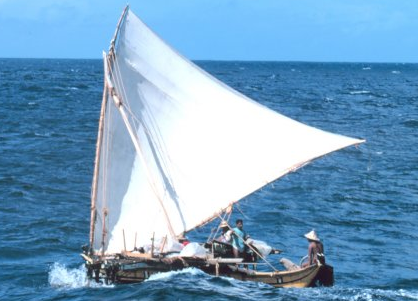
\includegraphics[scale=0.5]{sailboat.png}
%\end{center}
%\bigskip
%\noindent
A surface integral is like adding up all the wind on a sail.
In other words, we want to compute
$$\int\!\!\!\int{\bf F\cdot n}\,dA$$
where ${\bf F\cdot n}$ is the amount of wind normal to a tiny parallelogram $dA$.
The integral sums over the entire area of the sail.
Let $S$ be the surface of the sail parameterized by $x$ and $y$.
(In this model, the $z$ direction points downwind.)
By the properties of the cross product we have the following for the unit normal $\bf n$
and for $dA$.
$${\bf n}={ {{\partial S\over\partial x}\times{\partial S\over\partial y}}\over
 {\left|{\partial S\over\partial x}\times{\partial S\over\partial y}\right|}}\qquad
dA=\left|{\partial S\over\partial x}\times{\partial S\over\partial y}\right|\,dx\,dy$$
Hence
$$\int\!\!\!\int{\bf F\cdot n}\,dA=\int\!\!\!\int{\bf F}\cdot
\left({{\partial S\over\partial x}\times{\partial S\over\partial y}}\right)\,dx\,dy$$

\noindent
For example, evaluate the surface integral
$$\int\!\!\!\int_S{\bf F\cdot n}\,d\sigma$$
where ${\bf F}=xy^2z{\bf i}-2x^3{\bf j}+yz^2{\bf k}$, $S$ is the surface
$z=1-x^2-y^2$, $x^2+y^2\le1$ and $\bf n$ is upper.\footnote{
Kaplan, {\it Advanced Calculus,} p. 313.}

\medskip
\noindent
Note that the surface intersects the $xy$ plane in a circle.
By the right hand rule, crossing $x$ into $y$ yields $\bf n$ pointing upwards hence
$${\bf n}\,d\sigma=\left({{\partial S\over\partial x}\times{\partial S\over\partial y}}\right)\,dx\,dy$$
The following Eigenmath code computes the surface integral.
The symbols $f$ and $h$ are used as temporary variables.

\medskip
\verb$z=1-x^2-y^2$

\verb$F=(x*y^2*z,-2*x^3,y*z^2)$

\verb$S=(x,y,z)$

\verb$f=dot(F,cross(d(S,x),d(S,y)))$

\verb$h=sqrt(1-x^2)$

\verb$defint(f,y,-h,h,x,-1,1)$

$${1\over48}\pi$$



\index{Green's theorem}

\noindent
Green's theorem tells us that
$$\oint P\,dx+Q\,dy=\int\!\!\!\int
\left({\partial Q\over\partial x}-{\partial P\over\partial y}\right)
dx\,dy$$

\noindent
Evaluate $\oint (2x^3-y^3)\,dx+(x^3+y^3)\,dy$ around the circle
$x^2+y^2=1$ using Green's theorem.\footnote{
Wilfred Kaplan, {\it Advanced Calculus, 5th Edition,} 287.}

\medskip
\noindent
It turns out that Eigenmath cannot solve the integral directly using
$x$ and $y$.
So instead we use polar coordinates.

\medskip
\verb$P=2x^3-y^3$

\verb$Q=x^3+y^3$

\verb$f=d(Q,x)-d(P,y)$

\verb$x=r*cos(theta)$

\verb$y=r*sin(theta)$

\verb$f=eval(f)$

\verb$defint(f*r,r,0,1,theta,0,2pi)$

$${3\over2}\pi$$

\medskip
\noindent
A few words of explanation are in order.
The line $f=eval(f)$ is necessary to update $f$ with the polar
substitutions for
$x$ and $y$.
The $defint$ integrand is $f{*}r$ because $r\,dr\,d\theta=dx\,dy$.



\subsection{Stokes' theorem}
\index{Stokes' theorem}
Stokes' theorem proves the following equivalence of line and surface
integrals.
%\bigskip
%\noindent
%$\displaystyle{\oint_C P\,dx+Q\,dy+R\,dz}$
%$$=
%\int\!\!\!\int_S
%\left({\partial Q\over\partial x}-{\partial P\over\partial y}\right)\,dx\,dy
%+
%\left({\partial R\over\partial y}-{\partial Q\over\partial z}\right)\,dy\,dz
%+
%\left({\partial P\over\partial z}-{\partial R\over\partial x}\right)\,dz\,dx
%$$
%
%\noindent
%Curve $C$ is the perimeter around $S$.
%The theorem can be also be written as
$$\oint P\,dx+Q\,dy+R\,dz
=\int\!\!\!\int_S(\mathop{\rm curl}{\bf F})\cdot{\bf n}\,d\sigma
$$
where ${\bf F}=(P,Q,R)$.
For $S$ parametrized by $x$ and $y$ we have
$${\bf n}\,d\sigma=\left(
{\partial S\over\partial x}\times{\partial S\over\partial y}
\right)dx\,dy$$
In many cases, converting an integral according to
Stokes' theorem can turn a difficult problem into an easy one.

\medskip
\noindent
Let ${\bf F}=(y,z,x)$ and let $S$ be the part of the paraboloid
$z=4-x^2-y^2$
that is above the $xy$ plane.
The perimeter of the paraboloid is the circle $x^2+y^2=2$.
Calculate both the line and surface integrals.
It turns out that we need to use polar coordinates so that {\it defint} can
succeed.

\medskip
\verb$--Surface integral$

\verb$z=4-x^2-y^2$

\verb$F=(y,z,x)$

\verb$S=(x,y,z)$

\verb$f=dot(curl(F),cross(d(S,x),d(S,y)))$

\verb$x=r*cos(theta)$

\verb$y=r*sin(theta)$

\verb$defint(f*r,r,0,2,theta,0,2pi)$

$$-4\pi$$

\verb$--Line integral$

\verb$x=2*cos(t)$

\verb$y=2*sin(t)$

\verb$z=4-x^2-y^2$

\verb$P=y$

\verb$Q=z$

\verb$R=x$

\verb$f=P*d(x,t)+Q*d(y,t)+R*d(z,t)$

\verb$f=circexp(f)$

\verb$defint(f,t,0,2pi)$

$$-4\pi$$



\subsection{Fran\c cois Vi\`ete}
Fran\c cois Vi\`ete was the first to discover an exact formula for $\pi$.
Here is his formula.
\begin{displaymath}
{2\over\pi}={\sqrt2\over2}\times{\sqrt{2+\sqrt2}\over2}\times
{\sqrt{2+\sqrt{2+\sqrt2}}\over2}\times\cdots
\end{displaymath}
%We can flip it around and write the formula like this.
%\begin{displaymath}
%\pi=2\times{2\over\sqrt2}\times{2\over\sqrt{2+\sqrt2}}\times
%{2\over\sqrt{2+\sqrt{2+\sqrt2}}}\times\cdots
%\end{displaymath}
Let $a_0=0$ and $a_{n}=\sqrt{2+a_{n-1}}$.
Then we can write
\begin{displaymath}
{2\over\pi}={a_1\over2}\times{a_2\over2}\times
{a_3\over2}\times\cdots
\end{displaymath}
%
Solving for $\pi$ we have
\begin{displaymath}
\pi=2\times{2\over a_1}\times{2\over a_2}\times{2\over a_3}\times\cdots=2\prod_{k=1}^\infty
{2\over a_k}
\end{displaymath}
%
Let us now use Eigenmath to compute $\pi$ according to Vi\`ete's formula.
Of course, we cannot calculate all the way out to infinity, we have to stop somewhere.
It turns out that nine factors are just enough to get six digits of accuracy.

\medskip
\verb$a(n)=test(n=0,0,sqrt(2+a(n-1)))$

\verb$float(2*product(k,1,9,2/a(k)))$

$$3.14159$$

\medskip
\noindent
The function $a(n)$ calls itself $n$ times so overall there are
54 calls to $a(n)$.
By using a different algorithm with temporary variables, we can get the
answer in just nine steps.

\medskip
\verb$a=0$

\verb$b=2$

\verb$for(k,1,9,a=sqrt(2+a),b=b*2/a)$

\verb$float(b)$

$$3.14159$$



\section*{Curl in tensor form}
The curl of a vector function can be expressed in tensor form as
$$\mathop{\rm curl}{\bf F}=\epsilon_{ijk}\,{\partial F_k\over\partial x_j}$$
where $\epsilon_{ijk}$ is the Levi-Civita tensor.
The following script demonstrates that this formula is equivalent
to computing curl the old fashioned way.

\medskip
\verb$-- Define epsilon.$

\verb$epsilon=zero(3,3,3)$

\verb$epsilon[1,2,3]=1$

\verb$epsilon[2,3,1]=1$

\verb$epsilon[3,1,2]=1$

\verb$epsilon[3,2,1]=-1$

\verb$epsilon[1,3,2]=-1$

\verb$epsilon[2,1,3]=-1$

\verb$-- F is a generic vector function.$

\verb$F=(FX(),FY(),FZ())$

\verb$-- A is the curl of F.$

\verb$A=outer(epsilon,d(F,(x,y,z)))$

\verb$A=contract(A,3,4) --sum across k$

\verb$A=contract(A,2,3) --sum across j$

\verb$-- B is the curl of F computed the old fashioned way.$

\verb$BX=d(F[3],y)-d(F[2],z)$

\verb$BY=d(F[1],z)-d(F[3],x)$

\verb$BZ=d(F[2],x)-d(F[1],y)$

\verb$B=(BX,BY,BZ)$

\verb$-- Are A and B equal? Subtract to find out.$

\verb$A-B$

$$\left(\matrix{0\cr0\cr0}\right)$$

\newpage

\noindent
The following is a variation on the previous script.
The product $\epsilon_{ijk}\,\partial F_k/\partial x_j$
is computed in just one line of code.
In addition, the outer product and the contraction across $k$
are now computed with a dot product.

\medskip
\verb$F=(FX(),FY(),FZ())$

\verb$epsilon=zero(3,3,3)$

\verb$epsilon[1,2,3]=1$

\verb$epsilon[2,3,1]=1$

\verb$epsilon[3,1,2]=1$

\verb$epsilon[3,2,1]=-1$

\verb$epsilon[1,3,2]=-1$

\verb$epsilon[2,1,3]=-1$

\verb$A=contract(dot(epsilon,d(F,(x,y,z))),2,3)$

\verb$BX=d(F[3],y)-d(F[2],z)$

\verb$BY=d(F[1],z)-d(F[3],x)$

\verb$BZ=d(F[2],x)-d(F[1],y)$

\verb$B=(BX,BY,BZ)$

\verb$-- Are A and B equal? Subtract to find out.$

\verb$A-B$

$$\left(\matrix{0\cr0\cr0}\right)$$



\section*{Quantum-harmonic-oscillator}
For total energy $E$, kinetic energy $K$ and potential energy $V$ we have
$$E=K+V$$
The corresponding formula for a quantum harmonic oscillator is
$$(2n+1)\psi=-{d^2\psi\over dx^2}+x^2\psi$$
where $n$ is an integer and represents the quantization of energy values.
The solution to the above equation is
$$\psi_n(x)=\exp(-x^2/2)H_n(x)$$
where $H_n(x)$ is the $n$th Hermite polynomial in $x$.
The following Eigenmath code checks $E=K+V$ for $n=7$.

\medskip
\verb$n=7$

\verb$psi=exp(-x^2/2)*hermite(x,n)$

\verb$E=(2*n+1)*psi$

\verb$K=-d(psi,x,x)$

\verb$V=x^2*psi$

\verb$E-K-V$

$$0$$



\subsection{Hydrogen wavefunctions}
\index{hydrogen wavefunctions}
Hydrogen wavefunctions $\psi$ are solutions to the differential equation
$${\psi\over n^2}=\nabla^2\psi+{2\psi\over r}$$
where $n$ is an integer representing the quantization of total energy and
$r$ is the radial distance of the electron.
The Laplacian operator in spherical coordinates is
$$\nabla^2={1\over r^2}{\partial\over\partial r}
\left(r^2{\partial\over\partial r}\right)
+{1\over r^2\sin\theta}{\partial\over\partial\theta}
\left(\sin\theta{\partial\over\partial\theta}\right)
+{1\over r^2\sin^2\theta}{\partial^2\over\partial\phi^2}$$
The general form of $\psi$ is
$$\psi=r^le^{-r/n}L_{n-l-1}^{2l+1}(2r/n)
P_l^{|m|}(\cos\theta)e^{im\phi}$$
where $L$ is a Laguerre polynomial, $P$ is a Legendre polynomial and
$l$ and $m$ are integers such that
$$1\le l\le n-1,\qquad -l\le m\le l$$
The general form can be expressed as the product of a radial
wavefunction $R$ and a spherical harmonic $Y$.
$$\psi=RY,\qquad R=r^le^{-r/n}L_{n-l-1}^{2l+1}(2r/n),\qquad
Y=P_l^{|m|}(\cos\theta)e^{im\phi}$$
The following code checks $E=K+V$ for $n,l,m=7,3,1$.

\medskip
\verb$laplacian(f)=1/r^2*d(r^2*d(f,r),r)+$

\verb$1/(r^2*sin(theta))*d(sin(theta)*d(f,theta),theta)+$

\verb$1/(r*sin(theta))^2*d(f,phi,phi)$

\verb$n=7$

\verb$l=3$

\verb$m=1$

\verb$R=r^l*exp(-r/n)*laguerre(2*r/n,n-l-1,2*l+1)$

\verb$Y=legendre(cos(theta),l,abs(m))*exp(i*m*phi)$

\verb$psi=R*Y$

\verb$E=psi/n^2$

\verb$K=laplacian(psi)$

\verb$V=2*psi/r$

\verb$simplify(E-K-V)$

$$0$$



\subsection{Space shuttle and Corvette}
The space shuttle accelerates from zero to 17{,}000 miles per hour
in 8 minutes.
A Corvette accelerates from zero to 60 miles per hour in 4.5 seconds.
The following script compares the two.

\medskip
\verb$vs=17000*"mile"/"hr"$

\verb$ts=8*"min"/(60*"min"/"hr")$

\verb$as=vs/ts$

\verb$as$

\verb$vc=60*"mile"/"hr"$

\verb$tc=4.5*"sec"/(3600*"sec"/"hr")$

\verb$ac=vc/tc$

\verb$ac$

\verb$"Time for Corvette to reach orbital velocity:"$

\verb$vs/ac$

\verb$vs/ac*60*"min"/"hr"$

\medskip
\noindent
Here is the result when the script runs.
It turns out that the space shuttle accelerates more than twice as fast as a
Corvette.

\medskip
$$a_s={\hbox{127500 mile}\over(\hbox{hr})^2}$$

$$a_c={\hbox{48000 mile}\over(\hbox{hr})^2}$$

\verb$Time for Corvette to reach orbital velocity:$

$$\hbox{0.354167 hr}$$

$$\hbox{21.25 min}$$



\newpage

\section{Built-in functions}

\section*{abs}
abs($x$) returns the absolute value or vector length of $x$.
The mag function should be used for complex $x$.

\medskip
{\tt P=(x,y)}

{\tt abs(P)}

$$(x^2+y^2)^{1/2}$$

\section*{adj}
adj($m$) returns the adjunct of matrix $m$.

\section*{and}
and($a,b,\ldots$) returns the logical ``and'' of predicate expressions.

\section*{arccos}
arccos($x$) returns the inverse cosine of $x$.

\section*{arccosh}
arccosh($x$) returns the inverse hyperbolic cosine of $x$.

\section*{arcsin}
arcsin($x$) returns the inverse sine of $x$.

\section*{arcsinh}
arcsinh($x$) returns the inverse hyperbolic sine of $x$.

\section*{arctan}
arcttan($x$) returns the inverse tangent of $x$.

\section*{arctanh}
arctanh($x$) returns the inverse hyperbolic tangent of $x$.

\section*{arg}
arg($z$) returns the angle of complex $z$.

\section*{ceiling}
ceiling($x$) returns the smallest integer not less than $x$.

\section*{check}
check($x$) In a script, if the predicate $x$ is true then continue, else stop.

\section*{choose}
choose($n,k$) returns $\displaystyle\left({n \atop k}\right)$

\section*{circexp}
circexp($x$) returns expression $x$ with circular functions converted
to exponential forms.
Sometimes this will simplify an expression.

\section*{coeff}
coeff($p,x,n$) returns the coefficient of $x^n$ in polynomial $p$.

\section*{cofactor}
cofactor($m,i,j$) returns of the cofactor of matrix $m$ with respect to row $i$ and column $j$.

\section*{conj}
conj($z$) returns the complex conjugate of $z$.

\section*{contract}
\index{trace}
contract($a,i,j$) returns tensor $a$ summed over indices $i$ and $j$.
If $i$ and $j$ are omitted then indices 1 and 2 are used.
contract($m$) is equivalent to the trace of matrix $m$.

\section*{cos}
cos($x$) returns the cosine of $x$.
%If $x$ is a floating point number then $\cos(x)$ is evaluated numerically.

\section*{cosh}
cosh($x$) returns the hyperbolic cosine of $x$.

\section*{cross}
cross($u,v$) returns the cross product of vectors $u$ and $v$.

\section*{curl}
curl($u$) returns the curl of vector $u$.

\section*{d}
d($f,x$) returns the derivative of $f$ with respect to $x$.

\section*{defint}
defint($f,x,a,b,\ldots$)
returns the definite integral of $f$ with respect to $x$ evaluated from $a$ to $b$.
The argument list can be extended for multiple integrals.
For example, $d(f,x,a,b,y,c,d)$.

\section*{deg}
deg($p,x$) returns the degree of polynomial $p$ in $x$.

\section*{denominator}
denominator($x$) returns the denominator of expression $x$.

\section*{det}
det($m$) returns the determinant of matrix $m$.

\section*{do}
do($a,b,\ldots$) evaluates the argument list from left to right.
Returns the result of the last argument.

\section*{dot}
dot($a,b,\ldots$) returns the dot product of tensors.

\section*{draw}
draw($f,x$) draws the function $f$ with respect to $x$.

\section*{erf}
erf($x$) returns the error function of $x$.

\section*{erfc}
erf($x$) returns the complementary error function of $x$.

\section*{eval}
eval($f,x,n$) returns $f$ evaluated at $x=n$.

\section*{exp}
exp($x$) returns $e^x$.

\section*{expand}
expand($r,x$) returns the partial fraction expansion of the ratio of
polynomials $r$ in $x$.

\medskip
\verb$expand(1/(x^3+x^2),x)$

$${1\over x^2}-{1\over x}+{1\over x+1}$$

\section*{expcos}
expcos($x$) returns the cosine of $x$ in exponential form.

\medskip
{\tt expcos(x)}

$${1\over2}\exp(-ix)+{1\over2}\exp(ix)$$

\section*{expsin}
expsin($x$) returns the sine of $x$ in exponential form.

\medskip
{\tt expsin(x)}

$${1\over2}i\exp(-ix)-{1\over2}i\exp(ix)$$

\section*{factor}
factor($n$) factors the integer $n$.

\medskip
{\tt factor(12345)}

$$3\times 5\times 823$$

\medskip
\noindent
factor($p,x$) factors polynomial $p$ in $x$.
The last argument can be omitted for polynomials in $x$.
The argument list can be extended for multivariate polynomials.
For example, factor($p,x,y$) factors $p$ over $x$ and then over $y$.

\medskip
{\tt factor(125*x{\char94}3-1)}

$$(5x-1)(25x^2+5x+1)$$

\section*{factorial}
Example:

\medskip
{\tt 10!}

$$3628800$$

\section*{filter}
filter($f,a,b,\ldots$) returns $f$ with terms involving $a$, $b$, etc. removed.

\medskip
{\tt 1/a+1/b+1/c}

$${1\over a}+{1\over b}+{1\over c}$$

{\tt filter(last,a)}

$${1\over b}+{1\over c}$$

\section*{float}
float($x$) converts $x$ to a floating point value.

\medskip
{\tt sum(n,0,20,(-1/2){\char94}n)}

$$699051\over1048576$$

{\tt float(last)}

$$0.666667$$

\section*{floor}
floor($x$) returns the largest integer not greater than $x$.

\section*{for}
for($i,j,k,a,b,\ldots$) For $i$ equals $j$ through $k$ evaluate $a$, $b$, etc.

\medskip
{\tt x=0}

{\tt y=2}

{\tt for(k,1,9,x=sqrt(2+x),y=2*y/x)}

{\tt float(y)}

$$3.14159$$

\section*{gcd}
gcd($a,b,\ldots$) returns the greatest common divisor.

\section*{hermite}
hermite($x,n$) returns the $n$th Hermite polynomial in $x$.

\section*{hilbert}
hilbert($n$) returns a Hilbert matrix of order $n$.

\section*{imag}
imag($z$) returns the imaginary part of complex $z$.

\section*{inner}
inner($a,b,\ldots$) returns the inner product of tensors.
Same as the dot product.

\section*{integral}
integral($f,x$) returns the integral of $f$ with respect to $x$.

\section*{inv}
inv($m$) returns the inverse of matrix $m$.

\section*{isprime}
isprime($n$) returns 1 if $n$ is prime, zero otherwise.

\medskip
{\tt isprime(2{\char94}53-111)}

$$1$$

\section*{laguerre}
laguerre($x,n,a$) returns the $n$th Laguerre polynomial in $x$.
If $a$ is omitted then $a=0$ is used.

\section*{lcm}
lcm($a,b,\ldots$) returns the least common multiple.

\section*{leading}
leading($p,x$) returns the leading coefficient of polynomial $p$ in $x$.

\medskip
\verb$leading(5x^2+x+1,x)$

$$5$$

\section*{legendre}
legendre($x,n,m$) returns the $n$th Legendre polynomial in $x$.
If $m$ is omitted then $m=0$ is used.

\section*{log}
log($x$) returns the natural logarithm of $x$.

\section*{mag}
mag($z$) returns the magnitude of complex $z$.

\section*{mod}
mod($a,b$) returns the remainder of $a$ divided by $b$.

\section*{not}
not($x$) negates the result of predicate expression $x$.

\section*{nroots}
nroots($p,x$) returns all of the roots, both real and complex, of
polynomial $p$ in $x$.
The roots are computed numerically.
The coefficients of $p$ can be real or complex.

\section*{numerator}
numerator($x$) returns the numerator of expression $x$.
%\begin{itemize}
%\item[$\scriptstyle1$]{\tt numerator(a/b+b/a)}
%\item[$\scriptstyle2$]\hspace{50pt} $a^2+b^2$
%\end{itemize}

\section*{or}
or($a,b,\ldots$) returns the logical ``or'' of predicate expressions.

\section*{outer}
outer($a,b,\ldots$) returns the outer product of tensors.

\section*{polar}
polar($z$) converts complex $z$ to polar form.

\section*{prime}
prime($n$) returns the $n$th prime number, $1\le n\le10{,}000$.

\section*{print}
print($a,b,\ldots$) evaluates expressions and prints the results..
Useful for printing from inside a ``for'' loop.

\section*{product}
product($i,j,k,f$) returns $\displaystyle\prod_{i=j}^k f$

\section*{quote}
quote($x$) returns expression $x$ unevaluated.

\section*{quotient}
quotient($p,q,x$) returns the quotient of polynomials in $x$.

\section*{rank}
rank($a$) returns the number of indices that tensor $a$ has.
A scalar has no indices so its rank is zero.

\section*{rationalize}
rationalize($x$) puts everything over a common denominator.

\medskip
{\tt rationalize(a/b+b/a)}

$$a^2+b^2\over ab$$

\section*{real}
real($z$) returns the real part of complex $z$.

\section*{rect}
rect($z$) returns complex $z$ in rectangular form.

\section*{roots}
roots($p,x$) returns the values of $x$ such that the polynomial $p(x)=0$.
The polynomial should be factorable over integers.

\section*{simplify}
simplify($x$) returns $x$ in a simpler form.

\section*{sin}
sin($x$) returns the sine of $x$.

\section*{sinh}
sinh($x$) returns the hyperbolic sine of $x$.

\section*{sqrt}
sqrt($x$) returns the square root of $x$.

\section*{stop}
In a script, it does what it says.

\section*{subst}
subst($a,b,c$) substitutes $a$ for $b$ in $c$ and returns the result.

\section*{sum}
sum($i,j,k,f$) returns $\displaystyle\sum_{i=j}^k f$

\section*{tan}
tan($x$) returns the tangent of $x$.

\section*{tanh}
tanh($x$) returns the hyperbolic tangent of $x$.

\section*{taylor}
taylor($f,x,n,a$) returns the Taylor expansion of $f$ of $x$ at $a$.
The argument $n$ is the degree of the expansion.
If $a$ is omitted then $a=0$ is used.

\medskip
{\tt taylor(1/cos(x),x,4)}

$${5\over24}x^4+{1\over2}x^2+1$$

\section*{test}
test($a,b,c,d,\ldots$)
If $a$ is true then $b$ is returned else if $c$ is true then $d$ is returned, etc.
If the number of arguments is odd then the last argument is returned when all else fails.

\section*{transpose}
transpose($a,i,j$) returns the transpose of tensor $a$ with respect to indices $i$ and $j$.
If $i$ and $j$ are omitted then 1 and 2 are used.
Hence a matrix can be transposed with a single argument.

\medskip
{\tt A=((a,b),(c,d))}

{\tt transpose(A)}

$$\left(\matrix{a & c\cr b & d\cr}\right)$$

\section*{unit}
unit($n$) returns an $n\times n$ identity matrix.

\medskip
{\tt unit(2)}

$$\left(\matrix{1&0\cr0&1\cr}\right)$$

\section*{zero}
zero($i,j,\ldots$) returns a null tensor with dimensions $i$, $j$, etc.
Useful for creating a tensor and then setting the component values.


\printindex
\end{document}
